
\documentclass[a4paper]{article}

% ---------- packages
\usepackage[english]{babel}
\usepackage[utf8x]{inputenc}
\usepackage{amsmath}
\usepackage{graphicx}
\usepackage{float}
\usepackage{amssymb}

% ---------- to add line break in table
\newcommand{\specialcell}[2][c]{%
  \begin{tabular}[#1]{@{}c@{}}#2\end{tabular}}

% ---------- Title
\title{Using Nanoparticles to Detect Tumors}
\author{Sun Choi, Eric Groszman, Yunong Xu}

\begin{document}

\maketitle
\tableofcontents

% ---------- Abstract
\section*{Abstract}
Cancer is a major global health problem, and early detection greatly increases the chances for successful treatment. We worked to validate a new approach, which uses nanoparticles as biological markers and leverages their magnetic properties to detect tumors as small as 20,000 cells. We used simulated and true relaxometry data to measure the magnetic decay of nanoparticles. With these signals as input, we solved a linear program that minimizes the number of sources in the domain subject to equality between predicted signals and input signals. In our approach, the domain is assumed to be a discretized, NxN grid. This model returns predicted locations and intensities of the nanoparticle sources. Results from simulated and true data both show accurate results for single and multiple-source tests.

% ---------- Motivation/ Intro to problem
\section{Introduction to the problem}

More than 12 million people die of cancer globally per year [2]. Early cancer detection greatly increases the chances for successful treatment, and the best early detection methods today can catch tumors no smaller than 10 million cancer cells. 
In an effort to detect tumors at much earlier stages, we worked to validate a new approach that uses nanoparticles as biological markers and leverages their magnetic properties to detect tumors as small as 20,000 cells. 

First, antibody-coated nanoparticles are introduced into a sample [4]. The type of antibody that a nanoparticle is coated with determines the type of tumor it can attach to. After sufficient time for the nanoparticles to flow through the sample and attach to tumors that cross their path, a process called magnetic relaxometry is applied to the domain. 

In this process, the sample is put under a relaxometry machine (MRX II) that induces a magnetic pulse and measures the magnetic decay of the particles with seven sensors. With the signal data, we developed a model to locate where the tumor is. Previous attempts to solve this problem have not been sufficiently accurate with more complex multiple source scenarios, and it is our goal to come up with a more robust approach.

% ---------- Objective
\section{Objectives}
We sought to tackle three objectives for this project:

\begin{enumerate}
\item Develop a model to detect the location and intensity of nanoparticles based on relaxometry signals. 
\item Test the model with simulated and true data
\item Quantify the model’s runtime efficiency and sensitivity to signal error
\end{enumerate}

% ---------- Math model
\section{Formulating a Mathematical Model}

In order to break down the problem, there are a number of factors that must be considered:

\begin{enumerate}
\item Properties of the domain where the nanoparticles can be
\item Properties of nanoparticles, the sources to be measured
\item The relationship between the sensors and the domain
\end{enumerate}

The properties and model decisions for each of the three factors are explained in depth below and summarized at the end of this section.

% domain properties
\subsubsection*{Domain properties}
The true domain is a two-dimensional square area, analogous to the square phantom slides used for testing in the MRXII machine. This matters because only nanoparticles within this square domain will be detected. Note, however, that there are infinite possible nanoparticle locations within this square.

\subsubsection*{The Domain in our model}
We assume that the true domain is contained in a unit square. In our approach, we discretize the unit square to an N x N grid, with a total of $N^2$ gridpoints. By defining this grid, we limit the predicted nanoparticle locations returned by the model to the $N^2$ gridpoints, which is a finite number of locations. As N increases, the number of gridpoints increases exponentially. The goal is to choose a small enough N that still reasonably approximates the real scenario.

% nanoparticle properties
\subsubsection*{Nanoparticle properties}
In this problem, nanoparticles are being used as biological markers. The type of antibody that is coating the nanoparticle determines what type of tumor the nanoparticle can bind to. Compared to free-floating nanoparticles, bound nanoparticles have a significantly higher magnetic moment, or torque experienced due to an external magnetic field. As a result, it is expected that only particles that have "found" a tumor contribute to the decay signal. It is necessary to note that additional sources of error may add noise to the decay signal. Error handling techniques are discussed in the Procedure section.

\subsubsection*{Nanoparticles in our model}
In our model, we work under the assumption that nanoparticles that are bound to tumors are captured by the sensor signals. We expect the number of nanoparticles in the grid to be very low compared to the number of possible locations. Hence, we begin with a sparse minimization problem to enforce as few possible detected locations as possible. Additionally, in our model source intensities are scaled such that one nanoparticle has one unit of intensity. 

% sensor properties
\subsubsection*{Sensor-domain relationship}
There are seven SQUID sensors in the machine that measure the magnetic decay in the domain after each pulse. There is a physical relationship between a sensor and source locations called the \textbf{Biot-Savart Law} which gives the magnitude of the field felt by a sensor at a point in time, given a source location, the magnetic moment of the source, and sensor locations. However, we do not expect source locations or magnetic moment to be known variables. Our model takes the Biot-Savart Law and these shortcomings into account.

\subsubsection*{Sensor-domain relationship in our model}
We simplify the Biot-Savart Law to a inverse distance relationship between the sensors and the domain \cite{Liu}. With this simplification we are able to solve for multiple source locations and intensities without prior knowledge of magnetic moment. 

\subsubsection*{Summary}
The following table summarizes the main properties and decisions made about each factor: \\

$\begin{tabular}{|l|l|l|}\hline
  \textbf{Factor} & \textbf{True properties} & \textbf{Model Decision} \\ \hline  
  \text{Domain} & \text{Continuous unit square} & \text{Discretized N x N grid} \\ \hline  
  \text{Nanoparticles} & \specialcell{Bound nanoparticles and\\error contribute to signal} & \specialcell{Solution will be sparse\\ Intensity of one nanoparticle\\ is one unit} \\ \hline  
  \text{Sensor-domain relationship} & \text{Biot-Savart Law} & \text{Inverse Distance} \\ \hline
  
\end{tabular} $\\ \\

% ---------- Visual Representation of problem

\begin{figure}[H]
\centering
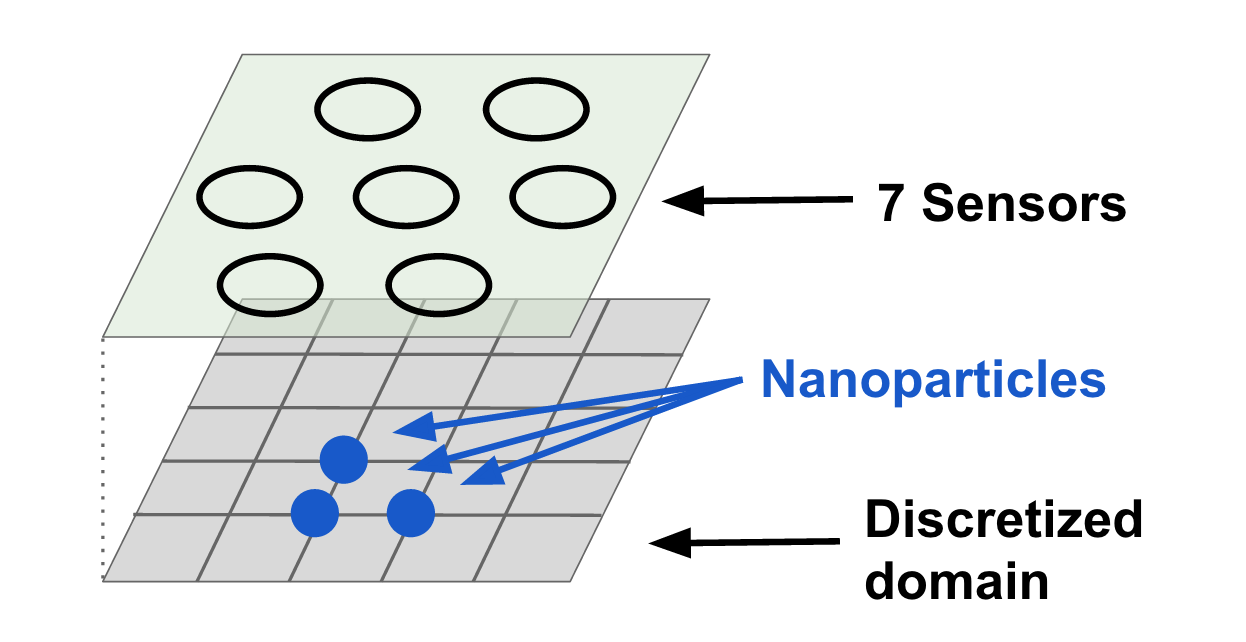
\includegraphics[width=1\textwidth]{machine_pic.png}
\caption{This is a visual representation of the problem. A sensor array is lifted off of a grid domain, and predicted nanoparticle locations can only occur at the gridpoints}
\label{Figure 1}
\end{figure}

With these model decisions in play, we can now state the Linear Program formulation.

% LP formulation
\subsection{Linear Program Formulation}

Our original LP takes the form of a sparse optimization problem that minimizes the $l_0$-norm of the solution vector x:

\begin{equation}
\centering
  \begin{array}{ll@{}r@{}r@{}l}
    \text{min} & \|x\|_0 \\[\jot]
    \text{s.t.}& Ax = b \\
    & \multicolumn{4}{l}{x \geq 0}
  \end{array}
\end{equation}

\subsubsection*{Matrix A}
A $\in \mathbb{R}^{7 \times N^2}$ encodes the sensor-domain relationship. \\Let $(X_i, Y_i, Z)$ be the position of sensor $i$ relative to the grid, $i$ = $1,2, \cdots , 7$. Let $(X_j, Y_j)$ be the location of gridpoint $j$, $j = 1,2, \cdots , N^2$. Then, the components of A are defined as: 
\[
A_{ij}=((X_{i}-X_{j})^2+(Y_{i}-Y_{j})^2+Z^2)^{-1}
\]

\subsubsection*{Vector x}
x $\in \mathbb{R}^{N^2 \times 1}$ is the solution vector containing the intensities at each gridpoint. Due to the expected sparsity of the problem, only a few entries in x are nonzero. A zero entry denotes zero intensity at a given gridpoint. The components of x are defined as: 
\[
x_j = \text{predicted intensity at gridpoint j, } j = 1,2, \cdots, N^2
\]

To visualize the grid, one can reshape x to an $N \times N$ matrix.

\subsubsection*{Vector b}
b $\in \mathbb{R}^{7 \times 1}$ is the input signal vector containing the signal intensity for each sensor. The components of b are defined as: 
\[
b_i = \text{signal magnitude of sensor i, }i = 1,2, \cdots, 7
\]

\subsubsection*{Reformulation of original LP}

The original problem statement minimizes the $l_0$-norm, which is defined as
\[
\|x\|_0 = \#(i|x_i \neq 0) \text{, or total number of nonzero elements in x}
\]

However, minimizing the $l_0$-norm of a non-binary $x$ is a difficult problem to solve. Given the nature of our problem, we approximate the $l_0$-norm with $l_1$ norm, defined as $\|x\|_1 = \sum\limits_{i} |x_i|$. Thus, we reformulate the original problem statement to:\\

\begin{equation}
\centering
  \begin{array}{ll@{}r@{}r@{}l}
    \text{min} & \sum\limits_{i} |x_i| \\[\jot]
    \text{s.t.}& Ax = b \\
    & \multicolumn{4}{l}{x \geq 0}
  \end{array}
\end{equation}

Note the lower bound on x. With this lower bound, there is no need to impose the absolute value. It is sufficient to minimize the sum of the entries in x. Because of these specific conditions, this equivalent formulation is adept to the numerous solvers designed to minimize $f^{T}x$ (in our case, $f^{T} = \vec{1}^{T}$:

\begin{equation}
\centering
  \begin{array}{ll@{}r@{}r@{}l}
    \text{min} & \sum\limits_{i} x_i \\[\jot]
    \text{s.t.}& Ax = b \\
    & \multicolumn{4}{l}{x \geq 0}
  \end{array}
\end{equation}

Lastly, we multiply $A$ by a scaling matrix $D$ \cite{Liu}. This is done simply to make the matrix $A$ better conditioned. Let $diag(v)$ denote a square diagonal matrix with the entries of vector $v$ in the diagonal. Then, D is defined as:
\[
D = diag(\|A_{:,j}\|_2), j = 1,2, \cdots, N^2 
\]

The LP with scaling matrix becomes: 

\begin{equation}
\centering
  \begin{array}{ll@{}r@{}r@{}l}
    \text{min} & \sum\limits_{i} x_i \\[\jot]
    \text{s.t.}& ADx = b \\
    & \multicolumn{4}{l}{x \geq 0}
  \end{array}
\end{equation}

\subsubsection*{Notes on Linear vs. Nonlinear approach:}

During the testing phase we weighed the advantages and disadvantages of approaching our model from a nonlinear approach. That is, minimizing a set of Biot-Savart equations against the retrieved decay signals at a point in time. There were some advantages and disadvantages to the nonlinear approach:\\

\noindent Advantages:
\begin{itemize}
\item Predicted location does not have to occur at a gridpoint
\item Potential to scale better than linear method
\end{itemize}
Disadvantages:
\begin{itemize}
\item Difficult to converge to one unique solution; there are many local minima especially with multiple sources
\item Need to specify the number of sources to detect on the domain
\end{itemize}

In the end, we pursued the linear approach primarily because it does not require specifying number of sources to detect.

% ---------- Procedure
\section{Procedure}

Our model tests involved two distinct scenarios. In the first, we simulated signal data to construct vector $b$ and the model was solved. In the second, true data was cleaned and stored in vector b. We describe the steps taken in both scenarios.

\subsection{Simulated Data Tests}

In summary, a grid is constructed. True source locations and intensities are placed on the grid and encoded in x*, a vector of true locations. Vector b is constructed by multiplying matrix A with x*. Noise is added to $b$. Then, the model solves for predicted solution x. Below are more detailed steps:

\begin{enumerate}
\item Choose gridsize N
\item Construct the N x N grid
\item Define sensor locations
\item Construct A, given the sensor locations and gridpoint locations
\item Construct scaling matrix D and multiply A with scaling matrix D: A = AD
\item Define the location and intensity of the true sources and store them in x*. For example, if we wish to place a single source at gridpoint n, we encode x* with $x_n^{*}$ = 1.
\item Construct noiseless signal vector b: b = Ax*
\item Add White Gaussian Noise to vector b. We used the built-in MATLAB function awgn, which adds a specified noise level to the input vector: b = awgn(b,level). level = 100 is no noise and level = 0 is drastic noise.

\end{enumerate}

With these steps, we have a scaled matrix A and a noisy signal vector b. The final step is to solve the LP for the predicted location and intensity vector x. The predicted solution can be compared to the true solution x*.

\subsubsection*{Notes on Noise}
It is important to note that in the true physical system, there are a number of factors that introduce signal noise. Three main factors are the magnetic field present in the background, the remnant field of the domain after each pulse is applied, and sensor error. In our simulated tests, we deliberately introduce White Gaussian noise into the input signal to introduce randomness into the model and to test the noise tolerance of the model.

\subsection{True Data Tests}
In order to test true data, steps 1-6 above are followed. However, steps 7-8 are ignored and a different procedure is taken to handle the true data:

\begin{enumerate}
\setcounter{enumi}{6}
\item Gather signal decays for each sensor in the sensor array
\item If for each sensor there is a set of decay signals corresponding to multiple decay pulses, average each sensor's decay set into one decay signal
\item For each sensor's decay, fit the decay points with a degree-two exponential function fit: 
\[
f(t) = a*e^{bt} + c*e^{dt}
\]
\item Isolate time point 0 for each fit. In other words, if we have seven fit functions $f_1(t), \cdots, f_7(t)$, take $f_1(0), \cdots, f_7(0)$. 
\item Store $f_1(0), \cdots, f_7(0)$ in signal vector b. These are the signal magnitudes for each sensor.
\item rescale signal vector b to the range [0 1]
\end{enumerate}

\subsubsection*{Notes on decay fits}
A number of decay fit methods were tested and the degree-two exponential function (exp2) was found to be the best fit function. Below is a summary of different decay fit methods with goodness-of-fit statistics ($R^2$ and root mean squared error):

\renewcommand{\arraystretch}{1.5}% Wider
\begin{center}
    \begin{tabular}{ | l | l | l | p{5cm} |}
    \hline
    Method & $R^{2}$ & RSME & Formula \\ \hline
    \textbf{exp2}  & .4899 & .0091 & $f(t) = a*e^{bt} + c*e^{dt}$ \\ \hline
    \textbf{poly2}  & .4396 & .0095 & $f(t) = at^{2} + bt + c$ \\ \hline    				
    \textbf{power2}  & .4458 & .0095 & $f(t) = at^{b} + c$\\ \hline    				
    \textbf{fourier2}  & .2430 & .0111 & $f(t) = a_0 + a_1cos(wt) + b_1sin(wt) + a_2cos(2wt) + b_2sin(2wt)$ \\ \hline
    \end{tabular}
\end{center}

\textbf{Comments:} We expect imperfect values for $R^{2}$ and RSME due to the variance of the oscillating points that the sensors capture. Therefore, even with the ideal fit there will be error in the fit equation. That said, the exp2 fit is the best fitting method, based on its goodness of fit coefficients and accurate characterization of the decay behavior that is captured by the SQUID sensor signals. 

\subsubsection*{Decay fits example}

\begin{figure}[H]
\centering
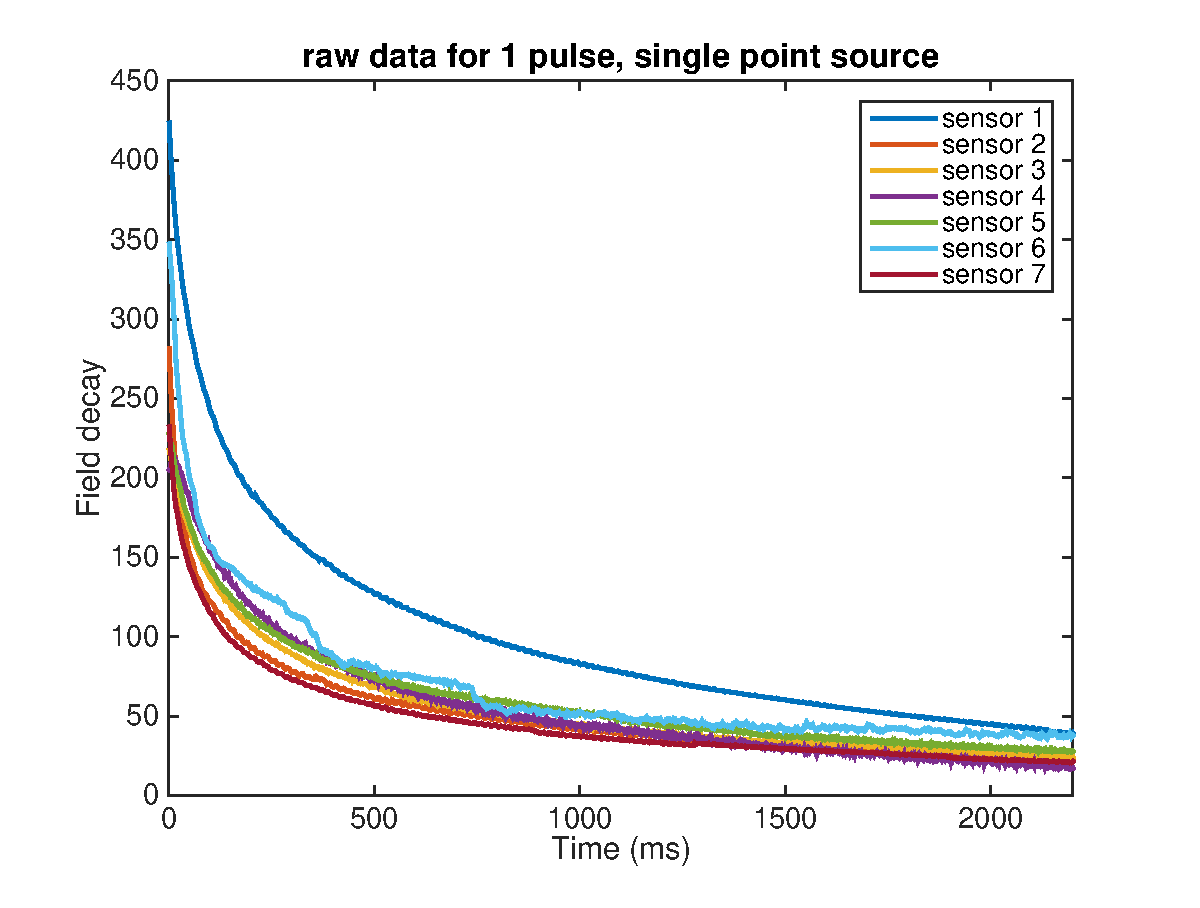
\includegraphics[width=1\textwidth]{raw_data}
\caption{Seven raw sensor decays for one pulse.}
\label{Figure 2}
\end{figure}

\begin{figure}[H]
\centering
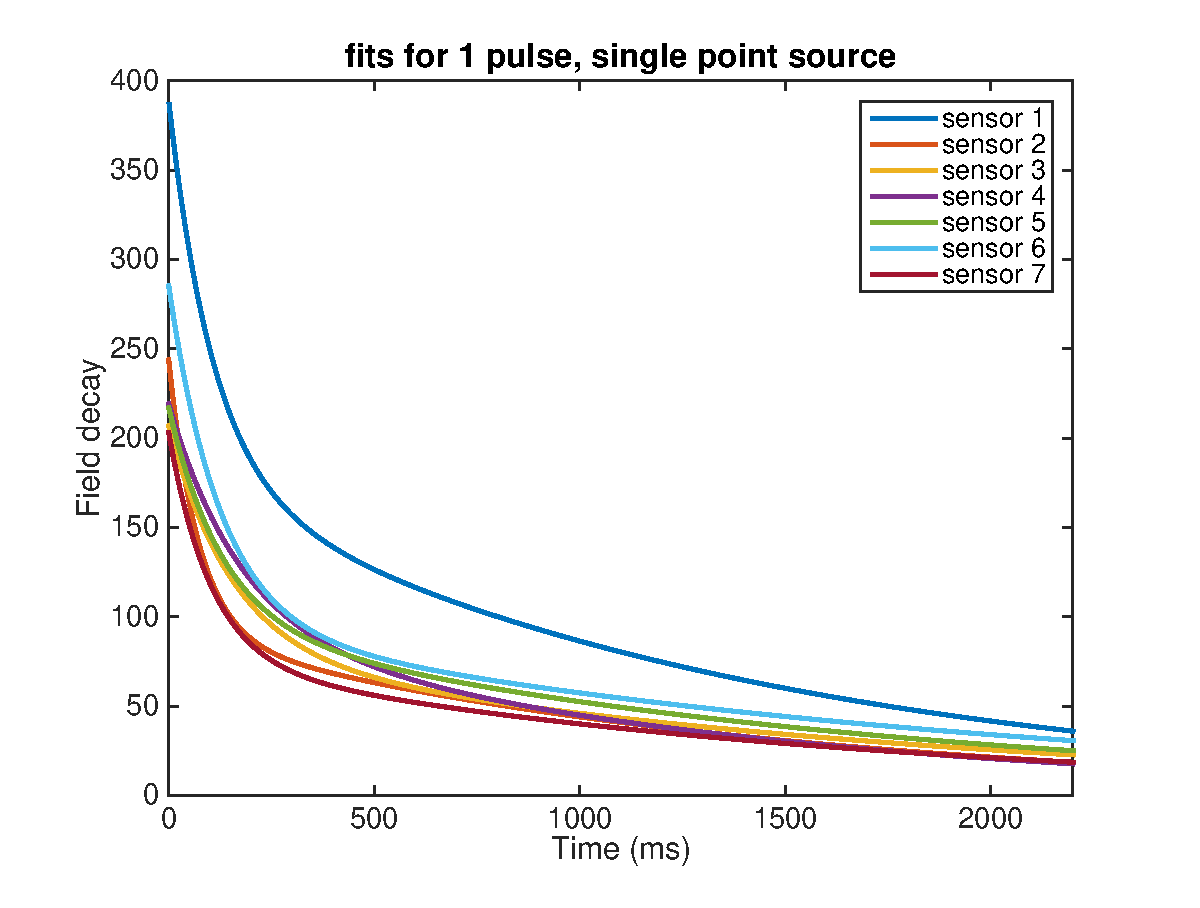
\includegraphics[width=1\textwidth]{fitted_data}
\caption{The fitted signals for each sensor. The fitted signal captures the decay pattern of each sensor. From this, we are able to characterize sensor signals with exp2 equation.}
\label{Figure 3}
\end{figure}

% ---------- Results
\section{Results}
 
Below are three tests based on simulated data and one test based on true data. In these figures, the white circles represent the sensor locations. The blue circles represent predicted source locations, and their size pertain to the predicted intensity at that location. Red circles are the true source location, with size marking intensity as well. However, the size of the red circles are made larger in order to be able to see both predicted and true sources. 
 
\subsection{Simulated Data Tests}
% do this to include an image
\begin{figure}[H]
\centering
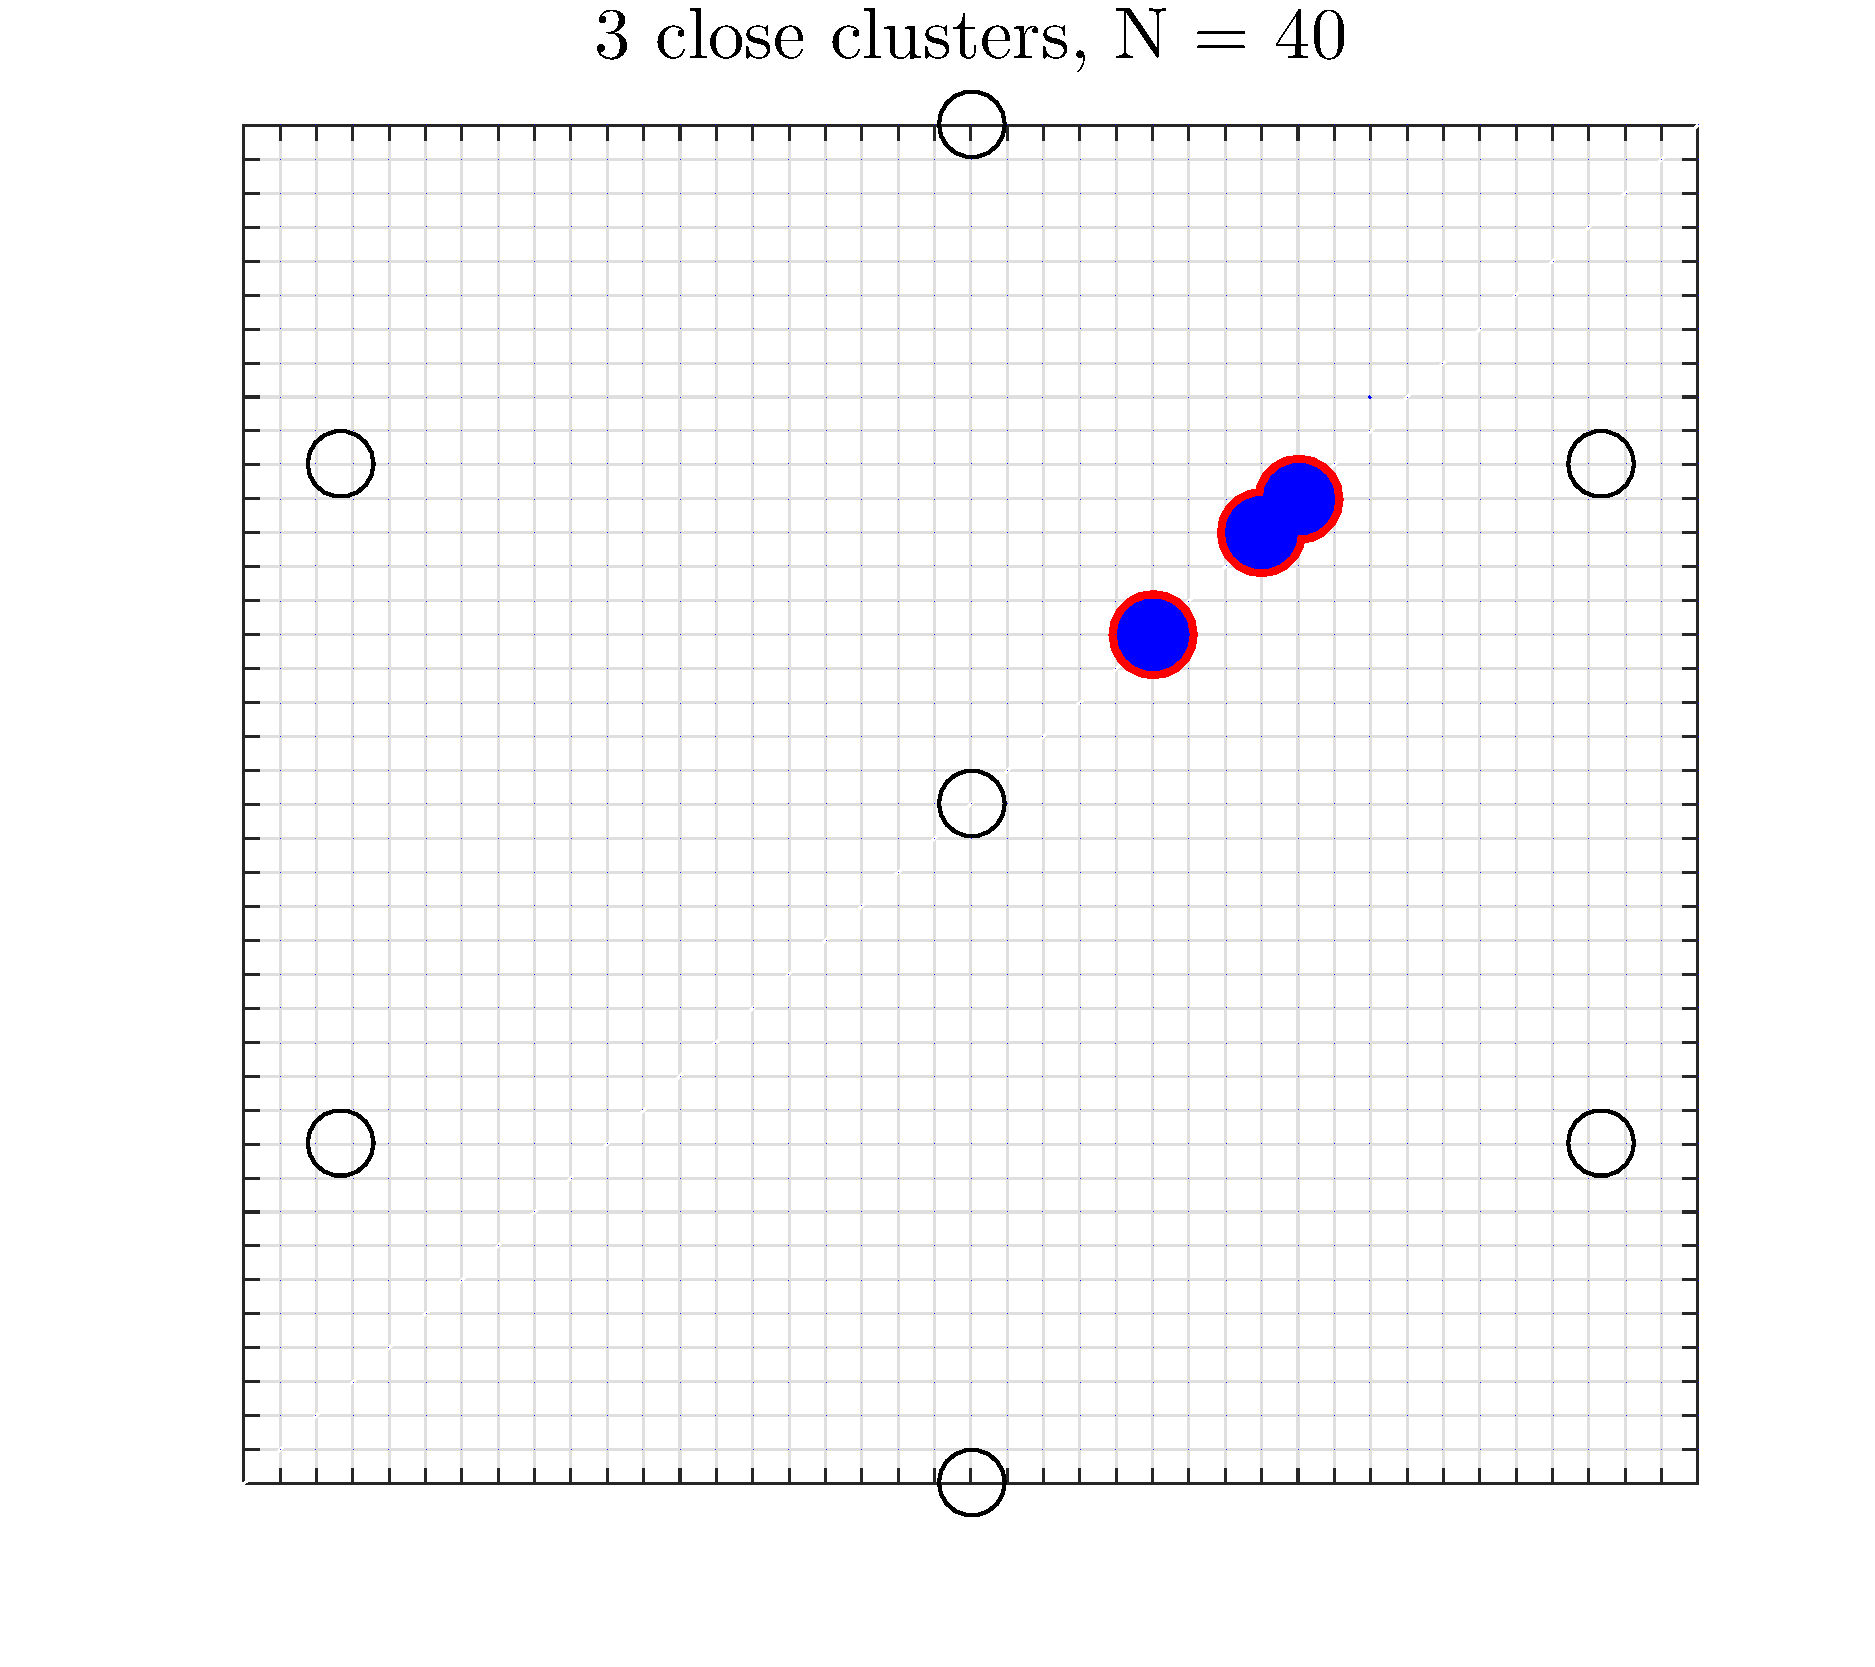
\includegraphics[width=.7\textwidth]{3_close_clusters_copy.pdf}
\caption{There are three clusters on the grid, equivalent to three single high-intensity sources. In this test we were looking to see if two close sources would be "seen" as one source by the sensor signals - but our model still distinguished between the two sources}
\label{Figure 4}
\end{figure}

\begin{figure}[H]
\centering
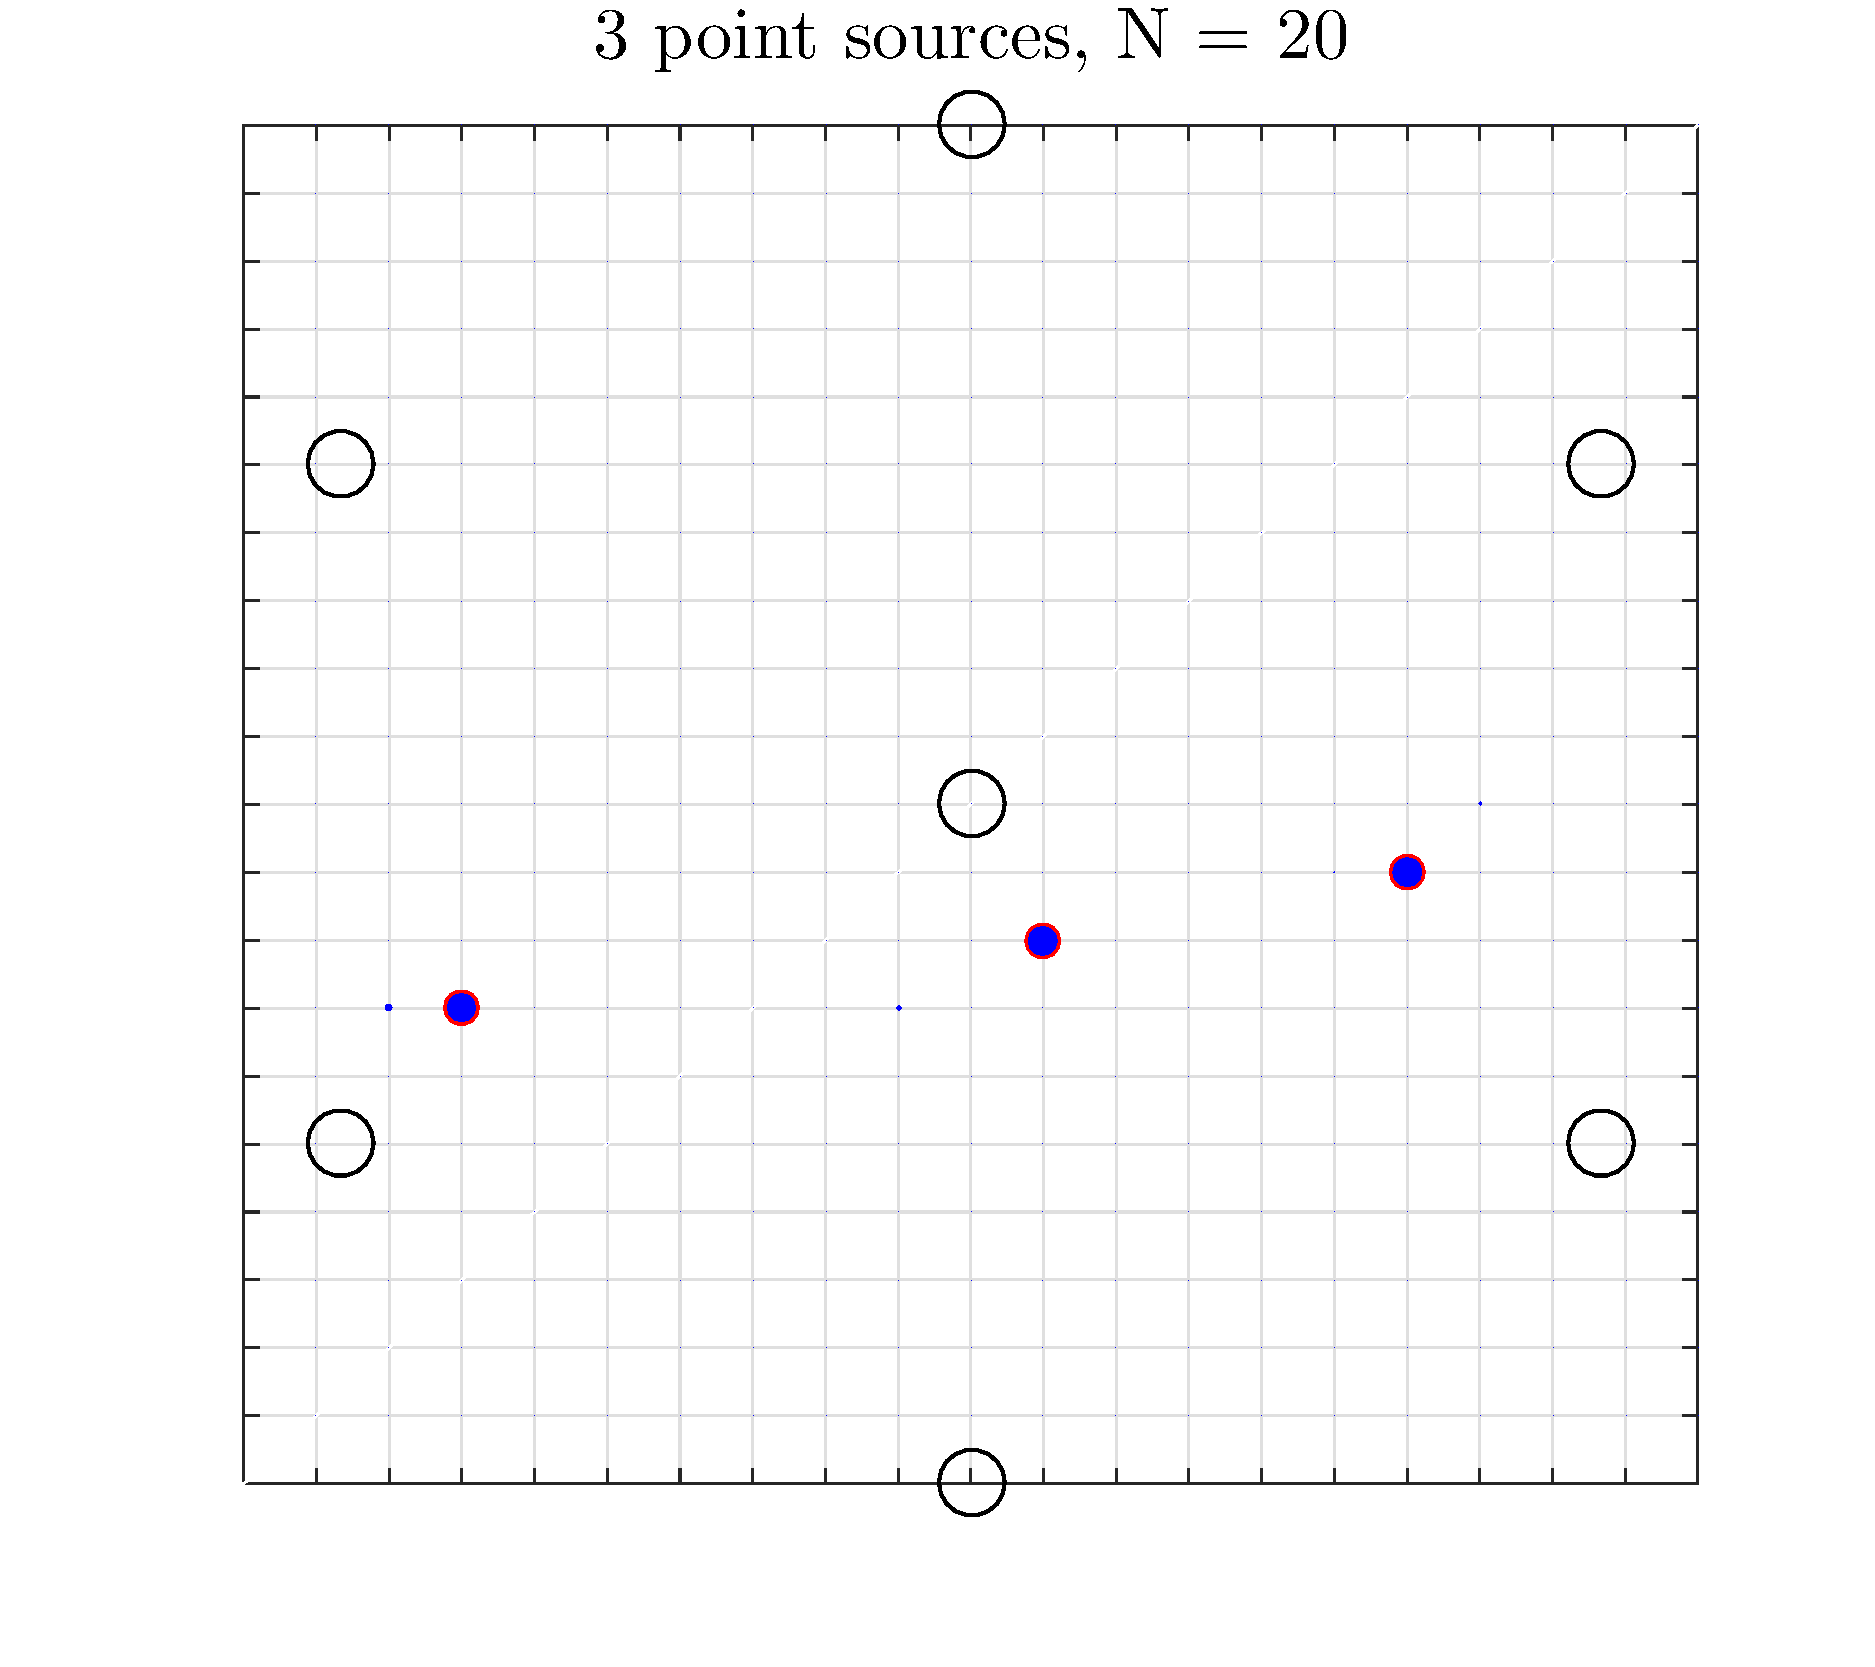
\includegraphics[width=.7\textwidth]{3_point_sources_copy.pdf}
\caption{In this second test, we placed three single sources of intensity one spread out from one another. Since each source has equal intensity it seemed very likely for the model to predict a location between the sources. The result, however, shows that the model was precise in distinguishing the three single sources.}
\label{Figure 5}
\end{figure}

\begin{figure}[H]
\centering
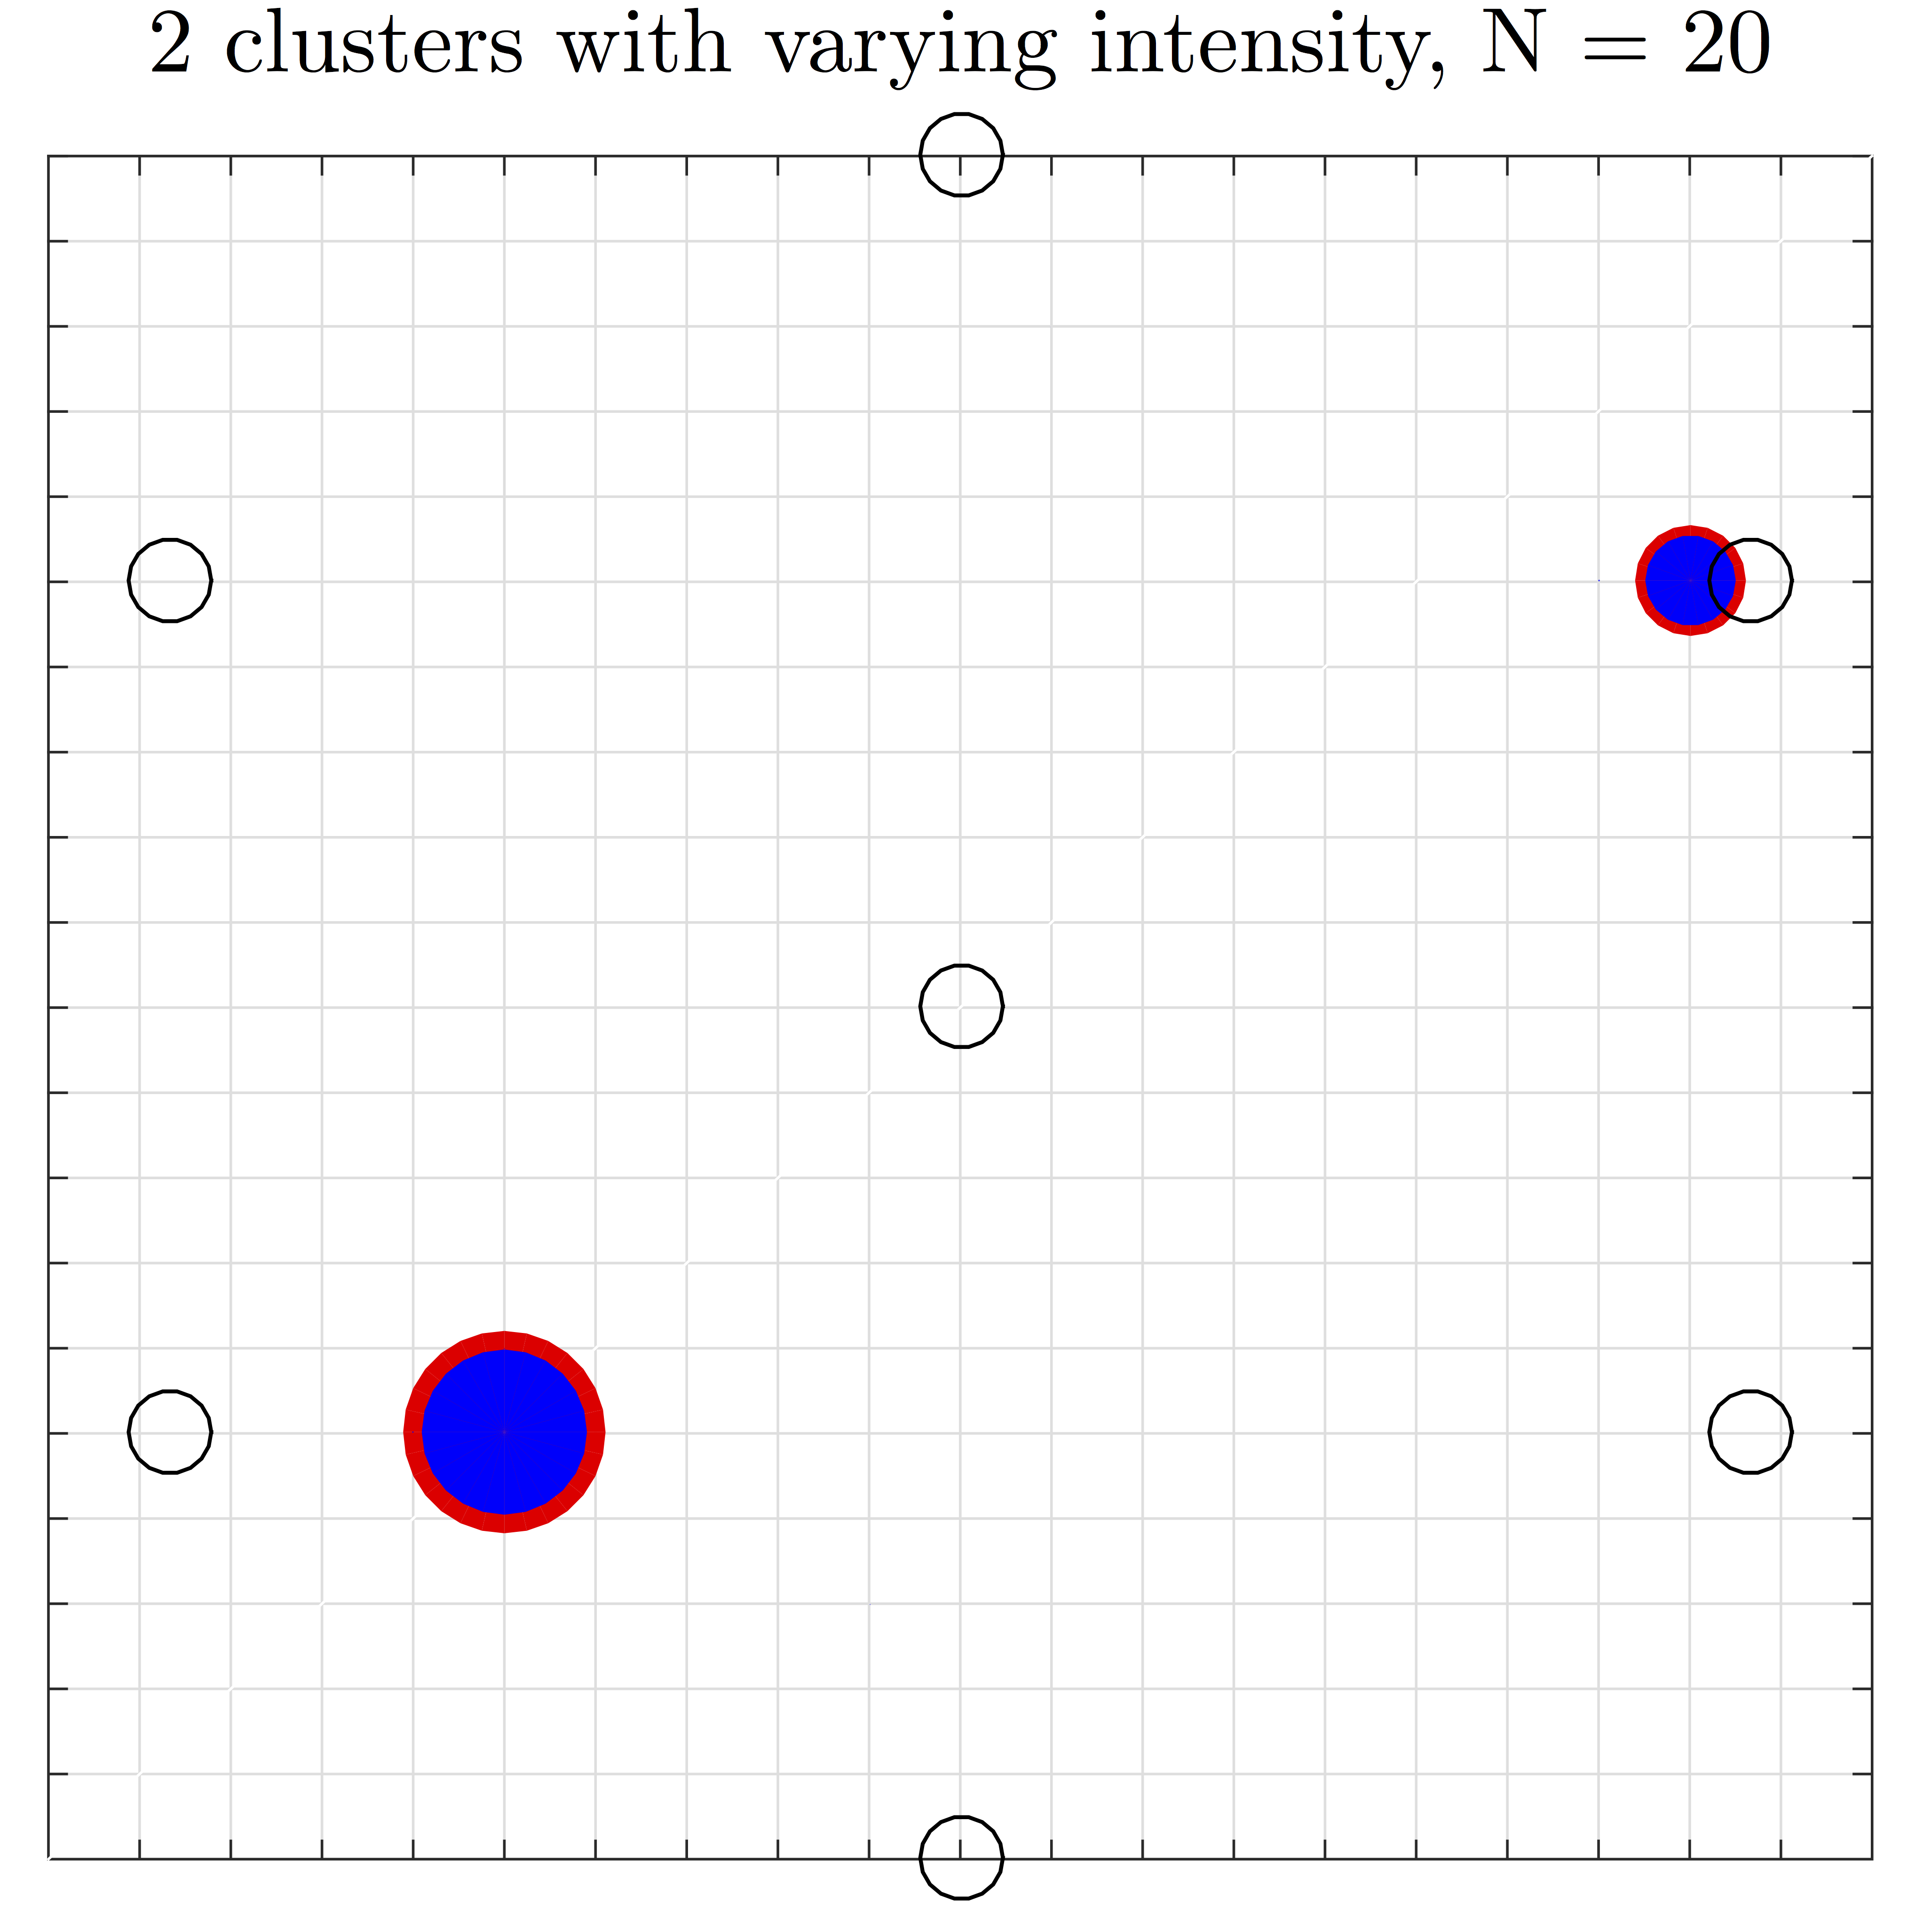
\includegraphics[width=.7\textwidth]{different_clusters_copy.png}
\caption{This test shows that a cluster with a high intensity does not affect the prediction of a separate, smaller cluster. We initially expected that the presence of the high intensity source would bring the predicted location of the smaller source towards the center.}
\label{Figure 6}
\end{figure}

\subsection{True data test}

\begin{figure}[H]
\centering
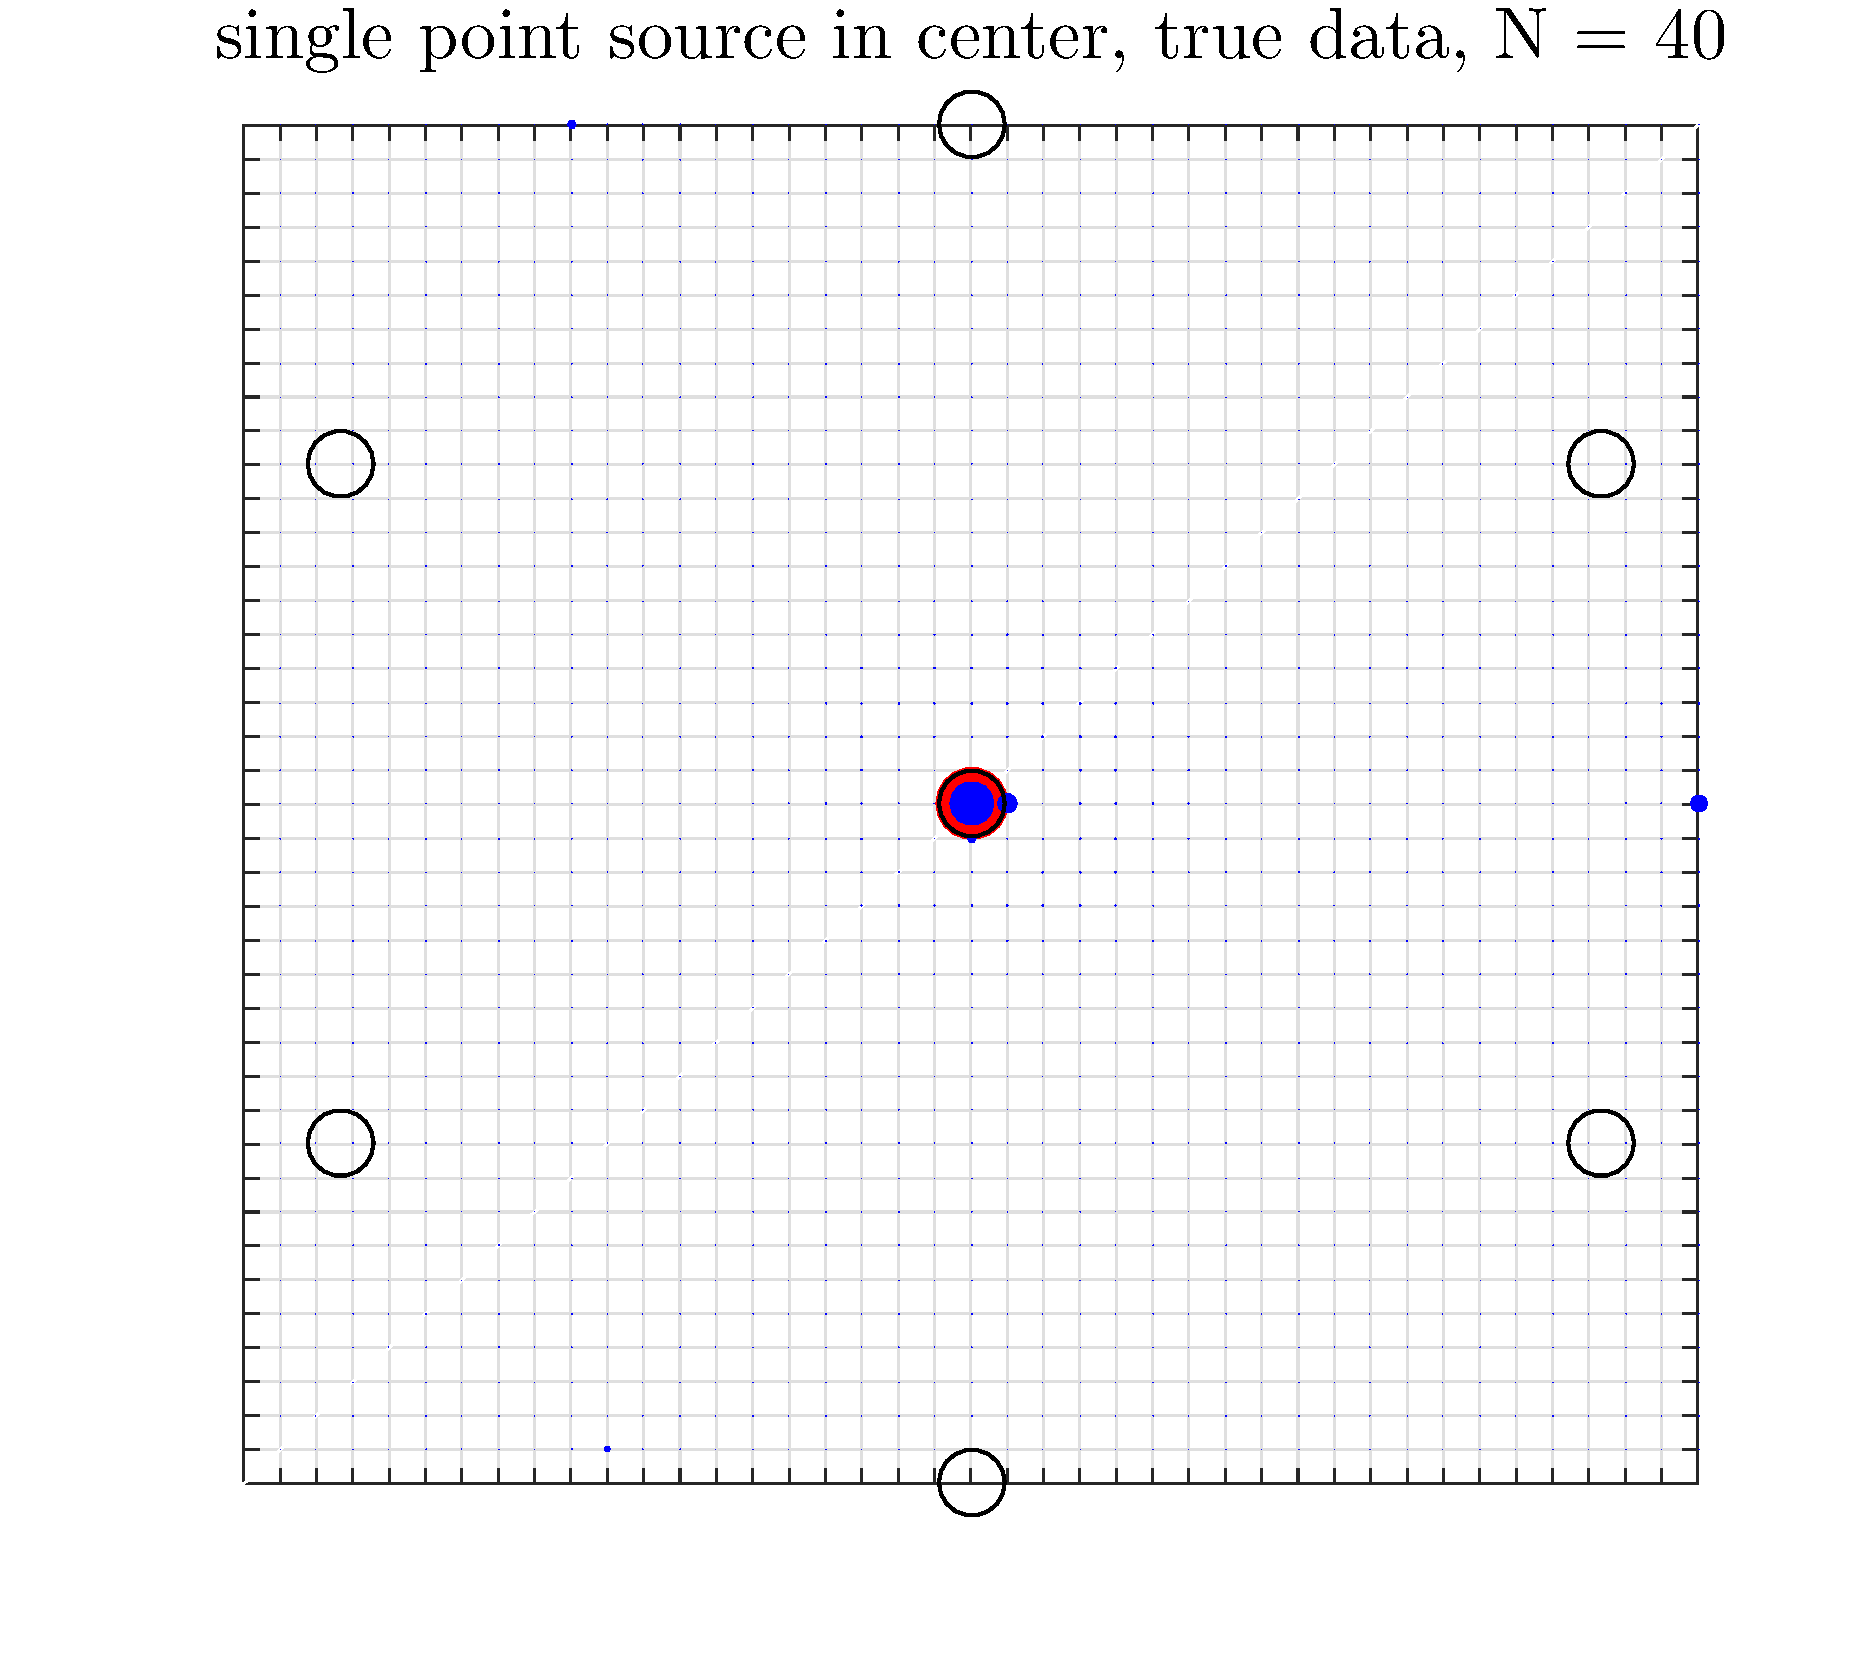
\includegraphics[width=.7\textwidth]{true_source_copy.pdf}
\caption{The result with real data is not as accurate as simulated data. While there is only one source, the sensors detect more than one source, shown as a small blue circle in the center with two blue dots on the edge, and a blue dot on the far right. However, the predicted intensities of three blue dots are smaller than the intensity of one nanoparticle.}
\label{Figure 7}
\end{figure}

\subsection{Noise tolerance test}

We wanted to take a look at our model's behavior as the input data becomes more noisy. Because there isn't a one-to-one correspondence between the number of true sources and number of predicted sources, it is difficult to quantify error between predicted and true solutions in a conventional way. We developed our own error-measuring approach, called Weighted Error. Weighted Error is calculated as follows:

\[ 
WE = \sum \limits_{j=1}^{N^2} d_j x_j.
\]

with $d_j$ representing the distance between predicted source $j$ and its nearest true source, and $x_j$ representing the intensity of predicted source j.

Below is Weighed error as a function of White Gaussian Noise:

\begin{figure}[H]
\centering
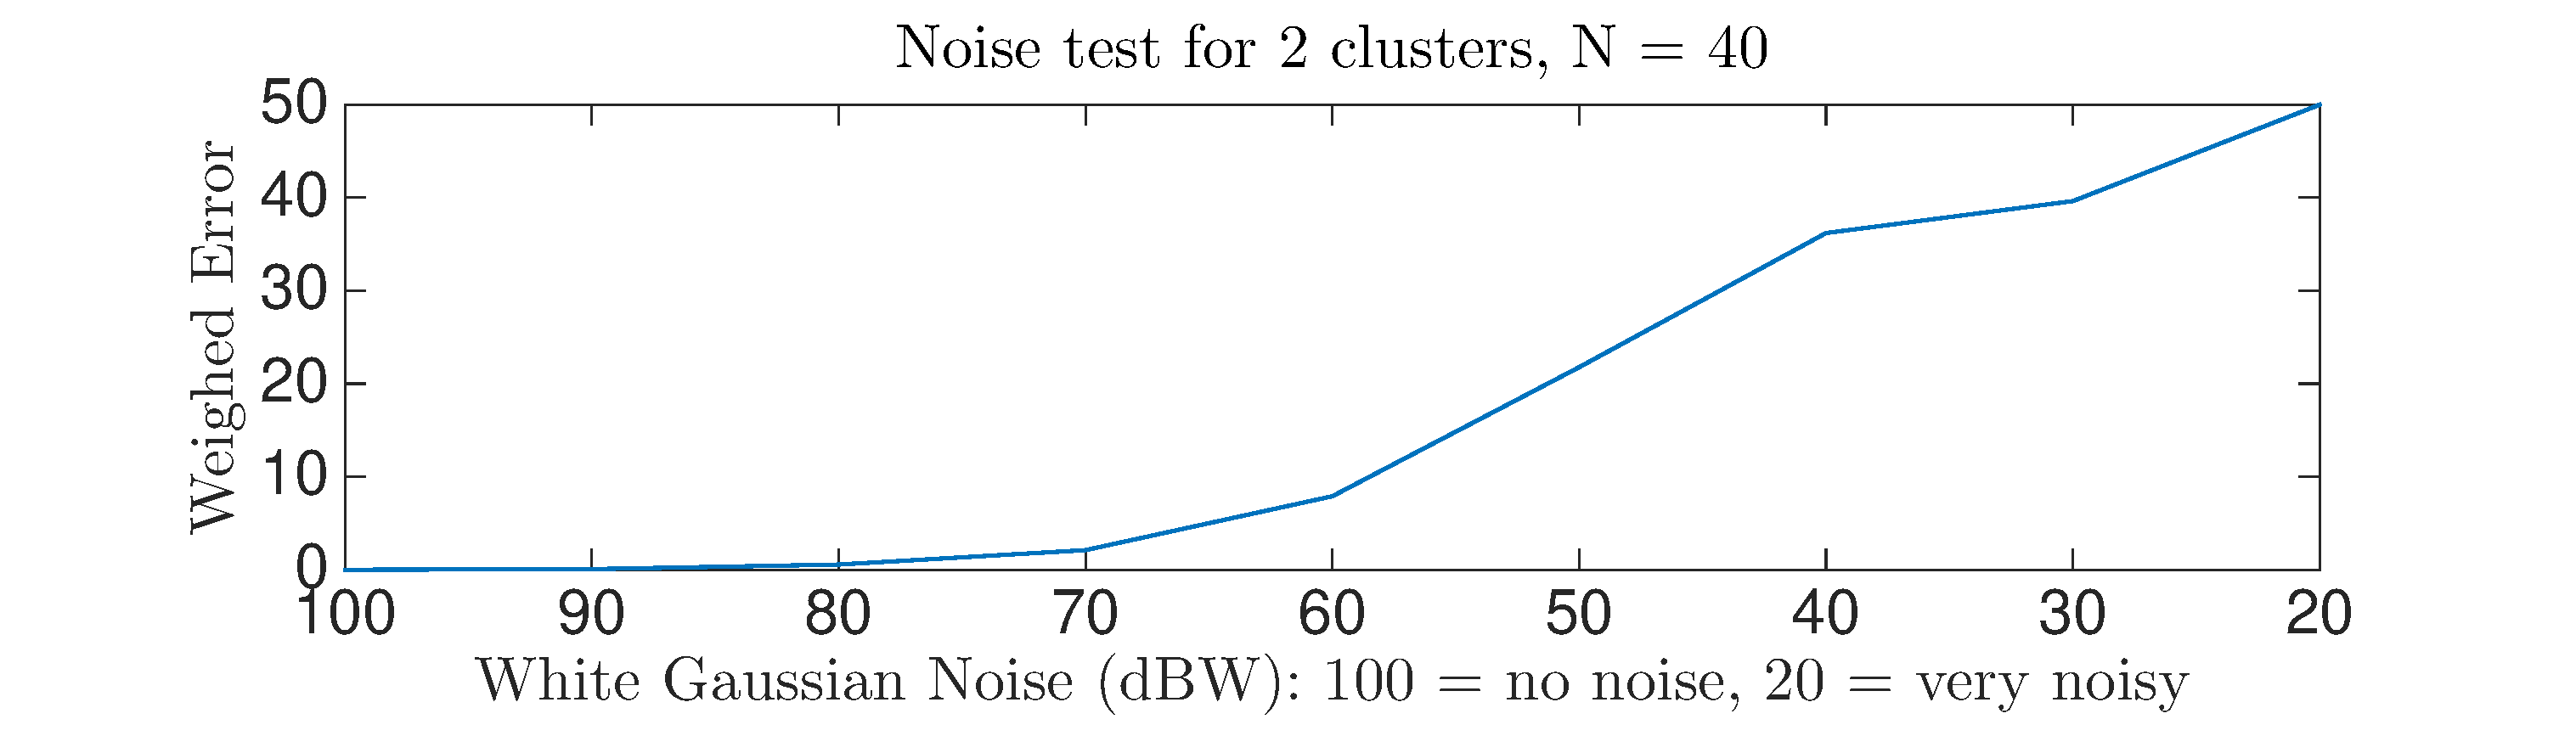
\includegraphics[width=1\textwidth]{noise_test}
\caption{The MRX II may operate in noisy environment. Thus we found an acceptable noise range that our model can intake by calculating weighted error. As you can see, the model begins to return inaccurate results starting at a noise level of 60 dBW.}
\label{Figure 8}
\end{figure}

\subsection{Computational Efficiency test}

We ran the model with a range of N, and for each N the model was timed. Below is a plot for $N = (2, 4, 8, 16, 32, 64, 128, 256)$

\begin{figure}[H]
\centering
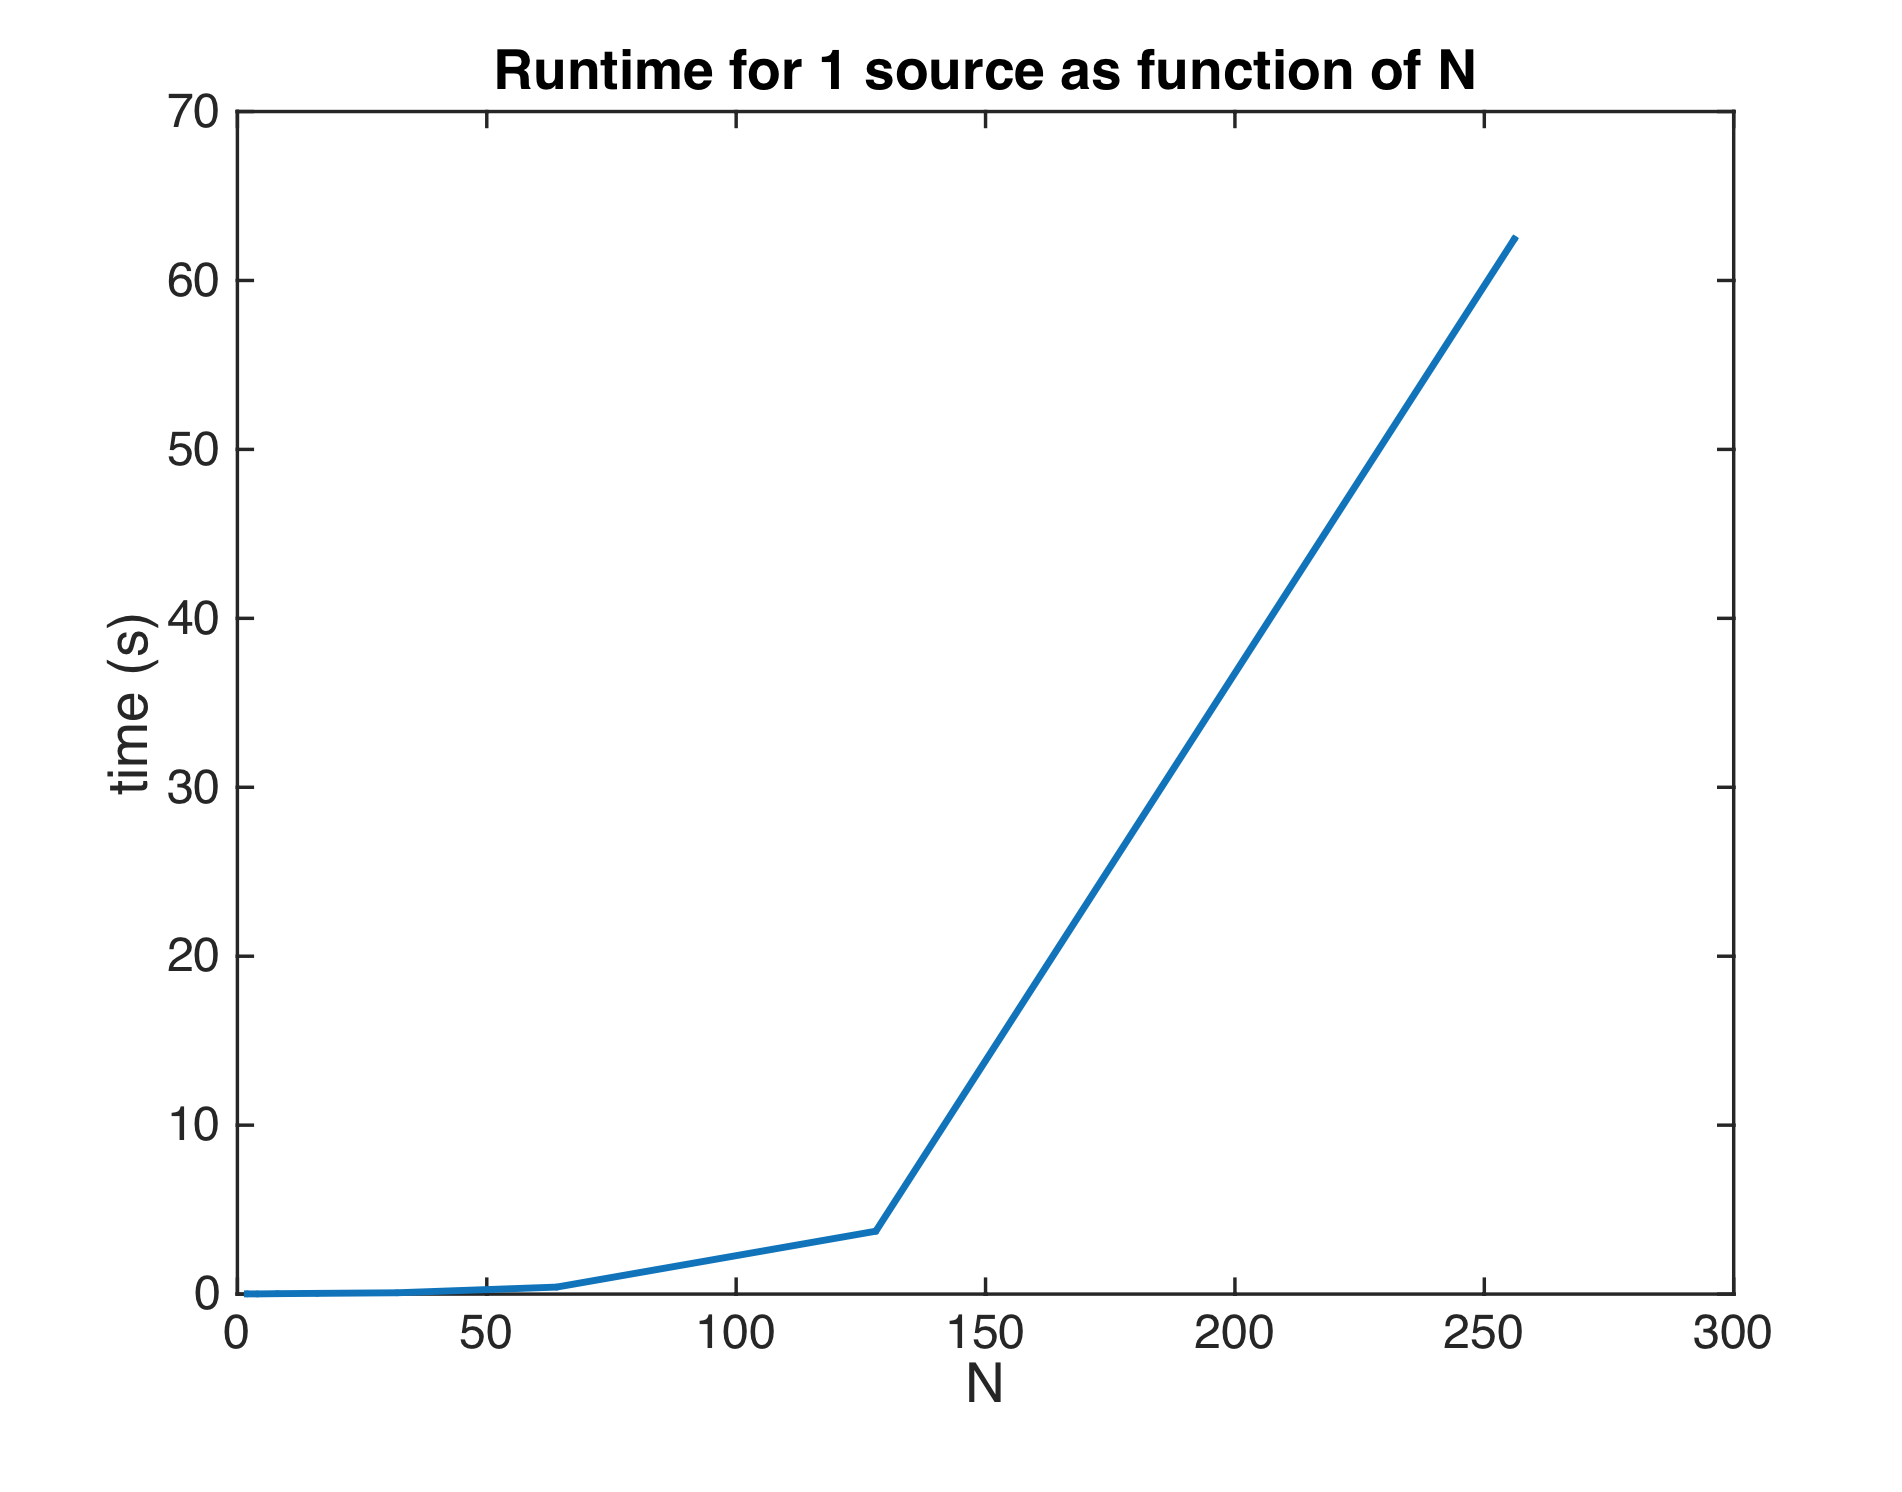
\includegraphics[width=.7\textwidth]{runtime_efficiency.png}
\caption{We tested the model with varying degrees of N to determine the runtime as the grid becomes finer. There is a rapid increase in the runtime at N = 128. However, the longest runtime is still around one minute.}
\label{Figure 9}
\end{figure} 

% ---------- Future Works
\section{Recommended expansions to model}

\subsection*{Mixed Linear Integer Program (MILP) Approach}

One drawback of our current LP approach is that it allows predicted sources to be any intensity. In reality, there is a (conditional) lower bound on signal intensity. Let lb and ub be scalars representing a lower bound and an upper bound on x, respectively. Then, using a MILP approach, x can be constrained as follows:
\[
x = \{x_i: x_i = 0, lb ≤ x_i ≤ ub\}
\]

In our case, lb = 1 (size of one nanoparticle) and ub = $\inf$. One way to formulate this MILP approach is by introducing a binary variable z with same size as x. Add additional constraints to original LP: \\

\[
x ≥ lb*z \: \rightarrow \: x - lb*z ≥ 0 
\]

\[
x ≤ ub*z \: \rightarrow \: x - ub*z ≤ 0 
\]

\[
z_i \in (0,1) \: i = 1, 2, … , N^2 
\]

With I representing the identity matrix, a complete MILP formulation is:

\begin{equation}
\centering
\begin{array}{ll@{}r@{}r@{}l}
    \text{min} & \|x\|_1 \\[\jot]
    \text{s.t.}& 
    \begin{bmatrix}
    AD & \vec{0}
	\end{bmatrix}
    \begin{bmatrix}
    x & z
	\end{bmatrix}
    = b \\
    \text{} & 
    \begin{bmatrix}
    -I & I(lb) \\
    I & -I(ub)
	\end{bmatrix}
    \begin{bmatrix}
    x & z
	\end{bmatrix}
    ≤ 0 \\ 
    & \multicolumn{4}{l}{x \geq 0} \\
    & \multicolumn{4}{l}{z \in (0,1)}
  \end{array}
\end{equation}

Other solvers allow the user to specify that x is a semicontinuous variable. If this is the case, solve the original LP formulation (4) with x defined as semicontinuous with the desired lower and upper bounds.

\subsection*{Expanding to three dimensions}
For our 3D domain, we cut the grid into multiple x-y planes and then find source location on that plane. However, due to the inverse distance, sensors may miscapture signal strengths. For example, when two sources have the same (X,Y) coordinates but different Z coordinates, the sensors may have difficulty predicting the layer that a source is on because different intensities can produce the same signal. 
To resolve this issue, we can measure signals with sensors in their original position, move the sensors by some amount, and measure signals again. 

\begin{figure}[H]
\centering
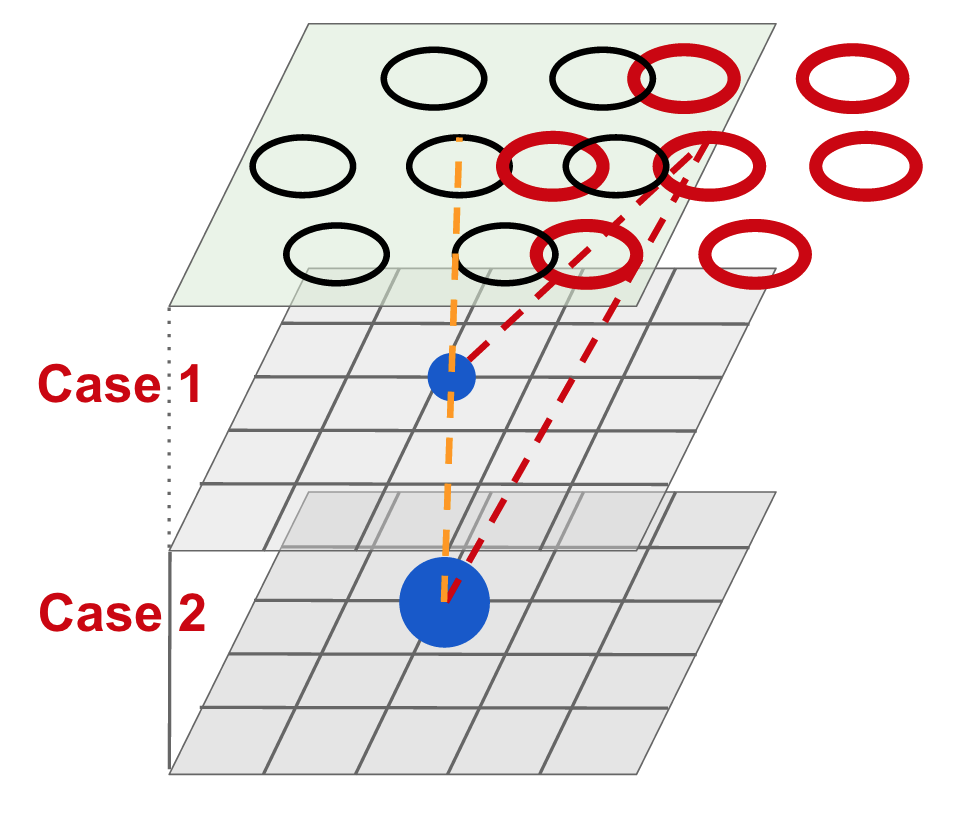
\includegraphics[width=.6\textwidth]{3d_model_fig.png}
\caption{here is the caption}
\label{Figure 10}
\end{figure}

The result is more sensor readings, causing matrix A to be larger (14 rows instead of 7) and vector b to be larger (14 entries instead of 7). 

\subsection*{Future Recommendation}

For future work, we recommend expanding our current model in the two directions suggested above. It is possible to introduce a semicontinuous variable x while also reformulating the linear program in three dimensions. 

Also it is very important to ensure data quality for true data tests. More specifically, the noise tolerance test for our model implies that when collecting true data, possible sources of error such as regular sensor maintenance and proper calibration of the MRXII must be carefully handled to minimize error in the collected data.

\section{Conclusion}

In conclusion, our Linear Program approach shows accurate predictions in both the simulated data tests and real data tests. In the simulated tests, the model is able to return accurate predictions for more complicated multiple source cases with varying intensities. 
In the real data test, the model predicts small peripheral sources with intensity less than one nanoparticle (not physically possible). However, the suggested MILP approach provides a better handling of the formulation and better predictions can be found. More generally, further strengthening the sparsity of the linear system could have positive effect on the model accuracy. For future work, expanding the model to three dimensions and further validating the model with real data will bring it one step closer to the big picture goal of providing patients with an efficient and effective way of detecting cancer at its very early stages.

\begin{thebibliography}{3} 
\bibitem{Liu} Liu, Kui, Source Localization on Two-Dimensional Grid, IEEE Globecom, 2011
\bibitem{Stewart} Stewart, Wild, World cancer report 2014. World Health Organization, 2014. Print.
\bibitem{Wang} Wang, Jia-Zhu,Magnetic Source Imaging Based on the Minimum-Norm Last-Squares Inverse,Brain Topography, Volume 5, Number 4, 1993 
\bibitem{Flynn} Flynn, Edward R., and Howard C. Bryant. "A Biomagnetic System for in Vivo Cancer Imaging." \emph{ Physics in Medicine and Biology} 50.6 (2005): 1273-293.

\end{thebibliography}


\end{document}

% ---- useful latex commands

% \begin{figure}
% \centering
% \includegraphics[width=0.3\textwidth]{frog.jpg}
% \caption{\label{fig:frog}This frog was uploaded via the project menu.}
% \end{figure}

% \begin{enumerate}
% \item Like this,
% \item and like this.
% \end{enumerate}
% \dots or bullet points \dots
% \begin{itemize}
% \item Like this,
% \item and like this.
% \end{itemize}

% \begin{document}
